% ======================================================================
%  Counting jobs, not shots
%  arXiv preprint, revtex4-2, single column
%  Build:  latexmk -pdf qaoa_job_budget.tex
%  Regenerate figures/tables first:  python3 make_figures.py && python3 make_tables.py
% ======================================================================
\documentclass[aps,prx,preprint,superscriptaddress,nofootinbib,longbibliography]{revtex4-2}

\usepackage{graphicx}
\usepackage{amsmath,amssymb}
\usepackage{booktabs}
\usepackage{algpseudocode}
\usepackage{xcolor}
\usepackage[colorlinks=true,allcolors=blue]{hyperref}
\usepackage{url}

\graphicspath{{figures/}}
%% auto-generated by make_tables.py -- do not edit
\newcommand{\swapgatemin}{1.28}
\newcommand{\swapgatemax}{1.37}
\newcommand{\swapdepthmin}{2.4}
\newcommand{\swapdepthmax}{2.8}
\newcommand{\bpsjobonesix}{0.808}
\newcommand{\bpsfinalsix}{0.913}
\newcommand{\serfinalsix}{0.922}
\newcommand{\jmatchsix}{3}
\newcommand{\njobssix}{8}
\newcommand{\bpsjoboneeight}{0.847}
\newcommand{\bpsfinaleight}{0.918}
\newcommand{\serfinaleight}{0.920}
\newcommand{\jmatcheight}{4}
\newcommand{\njobseight}{10}
\newcommand{\bpsjoboneten}{0.888}
\newcommand{\bpsfinalten}{0.926}
\newcommand{\serfinalten}{0.923}
\newcommand{\jmatchten}{5}
\newcommand{\njobsten}{12}
\newcommand{\bpsjobonetwelve}{0.915}
\newcommand{\bpsfinaltwelve}{0.928}
\newcommand{\serfinaltwelve}{0.916}
\newcommand{\jmatchtwelve}{12}
\newcommand{\njobstwelve}{12}
\newcommand{\ratiosix}{0.826}
\newcommand{\ratiosersix}{0.836}
\newcommand{\ratioctrlsix}{0.446}
\newcommand{\ratiounifsix}{0.451}
\newcommand{\enhsix}{10.7}
\newcommand{\ranksix}{1}
\newcommand{\nfeassix}{20}
\newcommand{\rhosix}{-0.97}
\newcommand{\rhoctrlsix}{+0.07}
\newcommand{\driftsix}{-0.034}
\newcommand{\ratioidealbpssix}{0.913}
\newcommand{\ratioidealsersix}{0.922}
\newcommand{\ratioeight}{0.772}
\newcommand{\ratiosereight}{0.740}
\newcommand{\ratioctrleight}{0.451}
\newcommand{\ratiounifeight}{0.456}
\newcommand{\enheight}{19.2}
\newcommand{\rankeight}{1}
\newcommand{\nfeaseight}{70}
\newcommand{\rhoeight}{-0.88}
\newcommand{\rhoctrleight}{+0.07}
\newcommand{\drifteight}{+0.043}
\newcommand{\ratioidealbpseight}{0.918}
\newcommand{\ratioidealsereight}{0.920}
\newcommand{\ratioten}{0.681}
\newcommand{\ratioserten}{0.662}
\newcommand{\ratioctrlten}{0.494}
\newcommand{\ratiouniften}{0.490}
\newcommand{\enhten}{16.8}
\newcommand{\rankten}{1}
\newcommand{\nfeasten}{252}
\newcommand{\rhoten}{-0.74}
\newcommand{\rhoctrlten}{-0.08}
\newcommand{\driftten}{-0.050}
\newcommand{\ratioidealbpsten}{0.926}
\newcommand{\ratioidealserten}{0.883}
\newcommand{\ratiotwelve}{0.614}
\newcommand{\ratiosertwelve}{0.601}
\newcommand{\ratioctrltwelve}{0.506}
\newcommand{\ratiouniftwelve}{0.505}
\newcommand{\enhtwelve}{11.0}
\newcommand{\ranktwelve}{2}
\newcommand{\nfeastwelve}{924}
\newcommand{\rhotwelve}{-0.45}
\newcommand{\rhoctrltwelve}{-0.00}
\newcommand{\drifttwelve}{+0.028}
\newcommand{\ratioidealbpstwelve}{0.923}
\newcommand{\ratioidealsertwelve}{0.891}
\newcommand{\totjobs}{102}
\newcommand{\totshots}{2\,624\,438}
\newcommand{\totqpu}{1329}
\newcommand{\totqpumin}{22.1}
\newcommand{\totwall}{6890}
\newcommand{\totwallmin}{115}
\newcommand{\wallratio}{5.2}
\newcommand{\etasix}{0.250}
\newcommand{\ntwoqsix}{90}
\newcommand{\etaeight}{0.403}
\newcommand{\ntwoqeight}{252}
\newcommand{\etaten}{0.631}
\newcommand{\ntwoqten}{540}
\newcommand{\etatwelve}{0.775}
\newcommand{\ntwoqtwelve}{990}
\newcommand{\etaa}{0.191}
\newcommand{\etab}{1.350}
\newcommand{\etamaxres}{0.029}
\newcommand{\costres}{1}
\newcommand{\twinratiodev}{0.06}
\newcommand{\twinfeasdev}{0.04}
\newcommand{\czerr}{0.264}
\newcommand{\pstarsix}{2}
\newcommand{\depthbestsix}{0.847}
\newcommand{\depthrunsix}{0.847}
\newcommand{\depthonesix}{0.739}
\newcommand{\enhbestsix}{12}
\newcommand{\enhonesix}{7}
\newcommand{\idealfivesix}{0.963}
\newcommand{\pstareight}{3}
\newcommand{\depthbesteight}{0.784}
\newcommand{\depthruneight}{0.784}
\newcommand{\depthoneeight}{0.659}
\newcommand{\enhbesteight}{22}
\newcommand{\enhoneeight}{6}
\newcommand{\idealfiveeight}{0.968}
\newcommand{\pstarten}{2}
\newcommand{\depthbestten}{0.758}
\newcommand{\depthrunten}{0.713}
\newcommand{\depthoneten}{0.619}
\newcommand{\enhbestten}{28}
\newcommand{\enhoneten}{8}
\newcommand{\idealfiveten}{0.961}
\newcommand{\pstartwelve}{2}
\newcommand{\depthbesttwelve}{0.727}
\newcommand{\depthruntwelve}{0.645}
\newcommand{\depthonetwelve}{0.588}
\newcommand{\enhbesttwelve}{30}
\newcommand{\enhonetwelve}{6}
\newcommand{\idealfivetwelve}{0.952}
\newcommand{\depthgaintwelve}{0.082}
\newcommand{\noiseawaremax}{0.011}
\newcommand{\depthjobs}{25}
\newcommand{\depthqpu}{152}
\newcommand{\repnbmean}{1.50}
\newcommand{\repnsmean}{5.75}
\newcommand{\repnbrange}{1--2}
\newcommand{\repnsrange}{3--8}
\newcommand{\repbpsfinal}{0.906}
\newcommand{\repserfinal}{0.910}
\newcommand{\repbpssd}{0.014}
\newcommand{\repsersd}{0.012}
\newcommand{\repbpsjobone}{0.843}
\newcommand{\repserjobone}{0.746}
\newcommand{\repmeasbps}{0.767}
\newcommand{\repmeasser}{0.754}
\newcommand{\repmeasbpssd}{0.011}
\newcommand{\repmeassersd}{0.015}
\newcommand{\repwins}{4}
\newcommand{\repjobs}{66}
\newcommand{\repqpu}{536}
\newcommand{\oosjobs}{91}
\newcommand{\oosres}{0.0}
\newcommand{\oosqpu}{688}
\newcommand{\alljobs}{193}
\newcommand{\allqpu}{2017}
\newcommand{\allqpumin}{34}
\newcommand{\allwall}{8576}
\newcommand{\allwallmin}{143}
\newcommand{\allwallratio}{4.3}
\newcommand{\allshots}{3\,738\,520}
\newcommand{\medianwall}{19.2}
\newcommand{\minwall}{10.7}
\newcommand{\maxwall}{1454}
\newcommand{\meanwall}{44}
\newcommand{\minshots}{5\,112}
\newcommand{\medianwallsmall}{14.4}
\newcommand{\wallnjobs}{193}
                       % auto-generated; every number below comes from the data

% flip to \extradatatrue once the depth-scan and replicate runs are in
\newif\ifextradata
\extradatatrue

\newcommand{\CVaR}{\mathrm{CVaR}}
\providecommand{\ket}[1]{|#1\rangle}
\providecommand{\bra}[1]{\langle#1|}
\newcommand{\ibmfez}{\texttt{ibm\_fez}}
\newcommand{\Ntwoq}{N_{2q}}
\newcommand{\Dtwoq}{D_{2q}}

\begin{document}

\title{Counting jobs, not shots: batched pattern search for the quantum
approximate optimization algorithm on cloud-accessed hardware}

\author{Muhammad Faryad}
\email{muhammad.faryad@lums.edu.pk}
\affiliation{Department of Physics, Lahore University of Management Sciences (LUMS),
Lahore 54792, Pakistan}

\date{\today}

\begin{abstract}
The cost of a variational quantum algorithm is almost always reported in circuit
evaluations or in shots. On a cloud-accessed processor neither is the quantity a user
actually spends: the unit that is charged and the unit that is queued is the
\emph{submitted job}. We measure that unit on IBM's \ibmfez. A job carries a fixed
overhead independent of its contents --- of order three seconds of metered processing time by
IBM's own documented estimator, and, in free-tier job mode, a measured round trip that never
once fell below \minwall\,s across the \alljobs\ jobs of this study, with a median of
\medianwall\,s and a tail reaching \maxwall\,s. Under this cost model an optimizer should be
judged by what it learns per job, and a serial optimizer that spends one job per function
evaluation pays that overhead $4p+2$ times over for what a batched iteration buys once. We therefore run a \emph{batched pattern search}, whose
entire iteration is known before any function value returns and which therefore probes
$4p+2$ points of the variational landscape in a single job, against COBYLA under an
identical budget of jobs \emph{and} shots. On four nested cardinality-constrained portfolio
instances of $6$, $8$, $10$ and $12$ assets, solved on \ibmfez\ and verified against exhaustive
enumeration, the batched search reaches after \emph{one} job a parameter quality that the
serial optimizer needs three to twelve jobs to match, an ordering that also survives four
independent initializations at $n=8$. The device ranks feasible portfolios in near-agreement with the exact ordering
(Spearman $\rho_s$ from \rhosix\ to \rhotwelve) and returns the true optimum as its most
probable feasible outcome at $n=6$, $8$ and $10$, and as its second most probable of
\nfeastwelve\ candidates at $n=12$, where shot noise on $\sim\!30$ counts no longer resolves
the leading few; a $\gamma=0$ control of identical depth shows
$\rho_s\approx0$, confirming that the ordering is not a device artefact. A single
two-parameter law, $\eta = 1-\exp[-(\etaa + \etab\times10^{-3}\Ntwoq)]$, reproduces the
effective depolarizing strength at all four sizes, and a $25$-job depth scan at classically
optimal parameters locates the device's optimal circuit depth at $p = 2$--$3$, beyond which
added layers cost more fidelity than they buy. The argument is not specific to QAOA: any
variational algorithm executed through a queue faces the same asymmetry between what a job
costs and what a job can carry.
\end{abstract}

\maketitle

% ======================================================================
\section{Introduction}
% ======================================================================

A variational quantum algorithm is a classical optimizer wrapped around a quantum
subroutine, and the conventional way to report its cost is to count the calls it makes to
that subroutine --- function evaluations, circuits, or shots. That accounting is natural if
the quantum computer sits on the desk. Almost none of them do. The overwhelming majority of
variational experiments are executed on processors reached through a cloud queue, and there
the resource a user spends is neither a shot nor an evaluation but a \emph{job}: a bundle of
circuits submitted as one unit, charged as one unit, and queued as one unit.

The distinction is not bookkeeping. A job has a fixed cost that its contents do not change.
We measure this cost directly in Sec.~\ref{sec:cost}: on IBM's 156-qubit Heron~r2 processor
\ibmfez, the metered quantum-processing time of a job is
\begin{equation}
  T_{\rm QPU} \;=\; 3.00\,\text{s} \;+\; \tau(\Dtwoq)\times N_{\rm shots},
  \label{eq:cost-preview}
\end{equation}
with $\tau$ of order $0.4\,$ms. A job carrying a single circuit at $5000$ shots therefore
spends more than half its metered budget on the fixed term. Wall-clock time is more lopsided
still, and unlike the metered figure it is something we measured directly: over the \alljobs\
jobs reported here the median round trip was \medianwall\,s, the fastest ever observed was
\minwall\,s, and the tail reached \maxwall\,s. Queueing and turnaround on shared quantum hardware have been
characterized before~\cite{ravi2021cloud,ravi2021adaptive,wu2024latency}, and the
implications for stochastic optimizers have been analyzed
theoretically~\cite{menickelly2023latency}; what has not been common practice is to design
and benchmark the optimizer with the job as the explicit unit of account.

\label{sec:intro-batching}%
Doing so changes which optimizer one should reach for. A job may carry many circuits, and in
Qiskit's primitive interface a single \emph{primitive unified bloc} (PUB) may carry an
arbitrary number of parameter vectors for one parameterized circuit. An optimizer can use
that capacity only to the extent that it can name points it wants evaluated \emph{before} it
sees any of the values, and methods differ enormously in how many points that is. At one
extreme, COBYLA~\cite{powell1994cobyla}, Nelder--Mead~\cite{nelder1965simplex} and
Powell~\cite{powell1964efficient} are sequential by construction once past their initial simplex
or direction set: each next point depends on the value just returned, so each evaluation is its
own job. In the middle, SPSA~\cite{spall1992spsa} names \emph{two} points per iteration --- the
$\pm c_k\Delta_k$ perturbations are both known before either value returns --- and a
parameter-shift gradient~\cite{mitarai2018qcl,schuld2019gradients} names all of its evaluations
at once; both are batchable, and we say so because the point is sometimes overlooked. At the far
end sits pattern search~\cite{torczon1997convergence,kolda2003directsearch,hough2001apps}, whose
\emph{entire} iteration --- the incumbent, a fixed stencil of trial points around it, and, in the
variant used here, one momentum probe --- is determined before any value returns. For a depth-$p$
QAOA ansatz with $2p$ parameters that is $4p+2$ landscape points in a single job. The claim of
this paper is not that batching is exotic; it is that points-per-round-trip is the axis along
which optimizers should be compared on queued hardware, and that it is rarely the axis
reported.

\paragraph*{What this paper contributes.}
\begin{enumerate}
\item \textbf{An explicit cost model for a hardware job} (Sec.~\ref{sec:cost}),
      instantiated from IBM's documented estimator for \ibmfez\ and used to budget every run in
      advance, together with the measured wall-clock cost of all \alljobs\ jobs. Both expose a
      fixed per-job overhead that the usual shot-based accounting hides, and we are explicit
      about which of the two is measured: the wall clock is, the metered time is not.
\item \textbf{A job-budgeted benchmarking protocol} (Sec.~\ref{sec:protocol}) in which the
      batched and the serial optimizer are given an identical number of jobs \emph{and} an
      identical number of shots, so that the only difference between the two arms is whether
      a job's shot budget is spent on one point of the landscape or spread across $4p+2$ of
      them. The intent is to remove shot count as an explanation, so that the comparison
      isolates allocation; Sec.~\ref{sec:protocol} discusses how much the serial arm can
      actually do with its $(4p+2)$-fold surplus, which on our own tuning data is little.
\item \textbf{A hardware demonstration at four sizes} (Sec.~\ref{sec:results}) on
      cardinality-constrained portfolio selection with $n = 6, 8, 10, 12$ assets, each small
      enough that the exact optimum and the exact ranking of every feasible portfolio are
      obtained by enumeration, so no claim rests on a heuristic reference.
\item \textbf{Controls that are usually missing}: a $\gamma = 0$ job of identical gate count
      and depth whose ideal output is exactly $\ket{+}^{\otimes n}$, which measures the noise
      floor; and a repeat of the first optimization job at the end of the run, which measures
      device drift across the comparison.
\item \textbf{A device characterization by-product}: the effective depolarizing strength
      inferred from the measured distributions follows a single two-parameter law in the
      two-qubit gate count across all four instances (Sec.~\ref{sec:noise}).
\item \textbf{A measured depth optimum} (Sec.~\ref{sec:depth}). Because the noiseless landscape
      is exactly optimizable at these sizes, the depth--noise trade-off can be measured with the
      optimizer removed: one job per $(n,p)$ at classically optimal parameters. The device
      optimum is $p = 2$--$3$, and reoptimizing against the noise model at fixed depth recovers
      none of the loss beyond it.
\item \textbf{A replicate study} (Sec.~\ref{sec:replicates}) repeating the $8$-asset comparison
      from four initializations, which puts a spread on the headline convergence claim.
\end{enumerate}

\paragraph*{Why this matters beyond QAOA.}
Nothing in the argument uses a property of QAOA. It uses two facts: that a job costs
something before it carries anything, and that some optimizers can name a batch of query
points in advance while others cannot. Both hold for every variational algorithm executed
through a queue. Variational eigensolvers sweep parameters the same way; quantum machine
learning trains parameterized circuits the same way; quantum kernel methods evaluate a Gram
matrix whose entries are mutually independent and therefore perfectly batchable; hardware
characterization, error-mitigation calibration and pulse tuning are parameter sweeps by
construction. The same asymmetry appears on trapped-ion and neutral-atom platforms reached
through the same kind of cloud interface. In every case the design question posed here is the
same one: given that you will pay a fixed price $J$ times, what is the most informative set
of $M$ points to put inside each of those $J$ payments? Pattern search is one answer, and a
deliberately simple one; model-based trust-region methods~\cite{sung2020models}, multistart
schemes~\cite{shaydulin2019multistart} and parameter-transfer
strategies~\cite{akshay2021concentration,galda2021transfer,sureshbabu2024parameter} are
others, and all of them become more attractive, not less, when the job rather than the
evaluation is the thing being counted.

The remainder of the paper is organized as a route that can be followed end to end. Section
\ref{sec:problem} states the optimization problem and its Ising form; Sec.~\ref{sec:circuit}
constructs the circuit; Sec.~\ref{sec:cost} measures what a job costs;
Sec.~\ref{sec:optimizer} states the optimizer; Sec.~\ref{sec:protocol} fixes the protocol and
its controls; Sec.~\ref{sec:results} reports the hardware results;
Sec.~\ref{sec:discussion} discusses limitations and consequences. Appendix~\ref{app:tuning}
records how every hyperparameter was chosen on a noise model \emph{before} any quantum
processing time was spent, and Appendix~\ref{app:repro} describes the released artifact.

% ======================================================================
\section{The problem and its Ising form}
\label{sec:problem}
% ======================================================================

We solve the discrete, cardinality-constrained form of Markowitz mean--variance portfolio
selection~\cite{markowitz1952portfolio}, a standard testbed for quantum
optimization~\cite{egger2020finance,herman2023finance,hodson2019portfolio,buonaiuto2023portfolio}.
Let $x_i \in \{0,1\}$ indicate that asset $i$ is held, $\mathbf r$ be the vector of expected
returns and $\Sigma$ the covariance matrix. With a hard budget of exactly $B$ assets, the
cost function is
\begin{equation}
  C(\mathbf x) \;=\; \lambda\, \mathbf x^{\mathsf T}\Sigma\,\mathbf x
  \;-\; \mathbf r^{\mathsf T}\mathbf x
  \;+\; \mu\Big(\textstyle\sum_i x_i - B\Big)^{2},
  \label{eq:costfn}
\end{equation}
the last term being the usual quadratic penalty that converts the constraint into a
QUBO~\cite{lucas2014ising,glover2019qubo}. Two coefficients in Eq.~\eqref{eq:costfn} deserve
more care than they usually receive, because both can silently trivialize the problem.

\emph{The risk aversion $\lambda$.} If $\lambda$ is small the quadratic term does nothing and
the ``optimization'' is a sort by expected return, which QAOA would then be credited with
solving. We remove the choice by fixing $\lambda$ so that, across the feasible set, the range
of the risk term equals the range of the return term,
\begin{equation}
  \lambda \;=\;
  \frac{\max_{\rm feas}(\mathbf r^{\mathsf T}\mathbf x) - \min_{\rm feas}(\mathbf r^{\mathsf T}\mathbf x)}
       {\max_{\rm feas}(\mathbf x^{\mathsf T}\Sigma\mathbf x) - \min_{\rm feas}(\mathbf x^{\mathsf T}\Sigma\mathbf x)} .
  \label{eq:lambda}
\end{equation}
Every instance below therefore has a risk-to-return spread ratio of exactly $1.000$, and the
optimum is genuinely a trade-off rather than a ranking.

\emph{The penalty $\mu$.} Too small and the global minimum of Eq.~\eqref{eq:costfn} is
infeasible; too large and $\mu$ dominates every Hamiltonian coefficient, the $ZZ$ couplings
become nearly uniform, and the ansatz spends its layers enforcing the Hamming weight instead
of discriminating among feasible portfolios. We scanned $\mu$ against the exactly optimized
ideal $p=2$ QAOA (Appendix~\ref{app:tuning}) and took the maximum of that scan, which lies at
$\mu \approx 0.05\times$ the spread of the penalty-free objective over the feasible set. The
resulting values are comfortable: at $n=6$ and $8$ the penalty-free objective already has a
feasible minimum, so any $\mu>0$ suffices, and at $n=10$ and $12$ the smallest penalty that makes
the ground state feasible is $5.4$ and $3.6$, against the chosen $12$ and $13$.

Under $x_i = (1-z_i)/2$, Eq.~\eqref{eq:costfn} becomes an Ising Hamiltonian
\begin{equation}
  \tilde H \;=\; \sum_i h_i Z_i + \sum_{i<j} J_{ij} Z_i Z_j ,
  \qquad C \;=\; s\,\tilde H + c ,
  \label{eq:ising}
\end{equation}
where the identity term has been removed and the coefficients rescaled so that
$\max(|h|,|J|) = 1$. The rescaling is not cosmetic: the pattern-search step size and the
shot-noise tolerance of Sec.~\ref{sec:optimizer} are both expressed in these units, and
without it they would have to be retuned for every instance. In these units the uniform
superposition has $\langle\tilde H\rangle = 0$ exactly, so a run that ends at a positive value
has done worse than doing nothing. Every notebook asserts that the diagonal of
Eq.~\eqref{eq:ising} reproduces Eq.~\eqref{eq:costfn} on all $2^n$ bitstrings before any
circuit is built.

The four instances are \emph{nested}: instance $n$ consists of the first $n$ assets of a
fixed twelve-asset table of large-capitalization US equities, with $B = n/2$. Any change in
the results across $n$ is therefore a property of the problem growing, not of four unrelated
problems. Their parameters and exact solutions are given in Table~\ref{tab:instances}.

\begin{table}[t]
\caption{The four nested instances. $r$(uniform) is the expected approximation ratio of the
uniform distribution over the feasible set, the baseline any method must beat. All quantities
are exact, from enumeration of all $2^n$ bitstrings.}
\label{tab:instances}
\begin{ruledtabular}
\begin{tabular}{cccccccc}
$n$ & $B$ & $\lambda$ & $\mu$ & $\binom{n}{B}$ & $C_{\min}$ & $C_{\max}^{\rm feas}$
 & $r$(uniform) \\
\hline
6 & 3 & 1.771 & 8 & 20 & -136.8 & 21.1 & 0.451 \\
8 & 4 & 1.653 & 9 & 70 & -161.1 & 23.3 & 0.456 \\
10 & 5 & 1.553 & 12 & 252 & -219.4 & 23.7 & 0.490 \\
12 & 6 & 1.360 & 13 & 924 & -243.3 & 26.0 & 0.505 \\
\end{tabular}
\end{ruledtabular}
\end{table}

We report three quantities throughout. The \emph{feasible probability mass} is the fraction
of shots with Hamming weight $B$; post-selecting on it is free error mitigation, since every
other bitstring is provably an error. The \emph{expected approximation ratio conditioned on
feasibility} is
\begin{equation}
  r \;=\; \frac{C_{\max}^{\rm feas} - \langle C\rangle_{\rm feas}}
                {C_{\max}^{\rm feas} - C_{\min}} ,
  \label{eq:ratio}
\end{equation}
an average over the whole post-selected distribution and therefore, unlike a best-of-$N$
figure, immune to inflation by taking more shots. The third is
$p(\text{optimum}\mid\text{feasible})$, reported as a multiple of the uniform value
$1/\binom{n}{B}$.

The optimizer, however, does not minimize Eq.~\eqref{eq:ratio}; it minimizes the conditional
value at risk~\cite{barkoutsos2020cvar}, $\CVaR_\alpha$, the mean energy of the lowest
$\alpha$ fraction of the sampled probability mass, at $\alpha = 0.5$. On a noisy device the
mean energy is dominated by the depolarized background while the tail still carries the
signal; $\alpha=0.5$ was selected in simulation (Appendix~\ref{app:tuning}) as the best
compromise between that effect and the shot noise of a short tail. Related tail-based and
filtering objectives are discussed in Ref.~\cite{amaro2022filtering}.

% ======================================================================
\section{Circuit synthesis on a chain}
\label{sec:circuit}
% ======================================================================

The cost Hamiltonian of Eq.~\eqref{eq:ising} is a \emph{complete} graph: every pair of assets
is coupled. The processor is heavy-hex. Handing the ansatz to a preset transpiler therefore
produces a routing solution whose depth is set by a SWAP heuristic and changes with the
random seed --- an unattractive property when the circuit is the independent variable of an
experiment.

We instead place the $n$ qubits on a single physical chain and realize all $\binom{n}{2}$
couplings with an odd--even transposition network
\cite{kivlichan2018lineardepth,ogorman2019swapnetworks,weidenfeller2022scaling}: at each of
$n$ steps, disjoint neighbouring pairs interact and then swap, so that after $n$ steps every
pair has met exactly once. Writing $\mathrm{RZZ}(\theta)\cdot\mathrm{SWAP}$ by hand as
\begin{equation}
  \texttt{cx}(a,b)\;\texttt{rz}(\theta,b)\;\texttt{cx}(b,a)\;\texttt{cx}(a,b),
  \label{eq:rzzswap}
\end{equation}
which is exact up to a global phase, costs three entangling gates per pair. The resulting
gate count is deterministic,
\begin{equation}
  \Ntwoq = 3p\binom{n}{2}, \qquad \Dtwoq = 3pn ,
  \label{eq:gatecount}
\end{equation}
independent of transpiler seed, and the final measurement permutation is tracked so that
classical bit $i$ always carries logical qubit $i$.

Emitting Eq.~\eqref{eq:rzzswap} explicitly rather than leaving it to the compiler matters:
Qiskit's two-qubit block consolidation cannot fuse gates carrying unbound
\texttt{Parameter}s, so a transpiled $\mathrm{RZZ}\cdot\mathrm{SWAP}$ costs five entangling
gates instead of three. Table~\ref{tab:circuit} and Fig.~\ref{fig:circuit} compare the
hand-built network against the preset pass manager at optimization level~3: the network uses
\swapgatemin--\swapgatemax\ times fewer two-qubit gates at
\swapdepthmin--\swapdepthmax\ times lower two-qubit depth. The chain itself is chosen at run
time by a beam search over simple paths of the coupling map that minimizes
$\sum -\log(1-\varepsilon)$ over the CZ and readout errors of the path, so that the circuit
sits on the best line the device has on the day, and the notebook asserts that the pass
manager did not move it. Each circuit is verified against the exact QAOA state vector before
submission.

\begin{figure}[t]
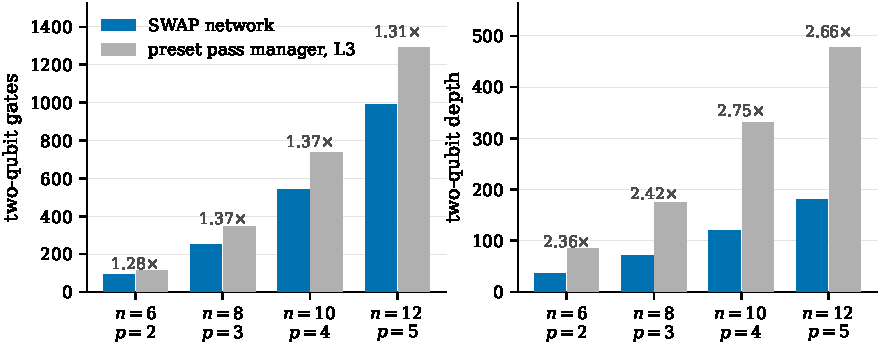
\includegraphics[width=\columnwidth]{fig_circuit.pdf}
\caption{Two-qubit gate count and two-qubit depth of the swap-network synthesis against
Qiskit's preset pass manager at optimization level~3, for the four circuits actually
submitted. Labels give the ratio.}
\label{fig:circuit}
\end{figure}

\begin{table}[t]
\caption{Circuit resources on \ibmfez. The swap-network columns follow
Eq.~\eqref{eq:gatecount} exactly; the preset columns depend on the transpiler seed.}
\label{tab:circuit}
\begin{ruledtabular}
\begin{tabular}{cccccccc}
& & \multicolumn{2}{c}{swap network} & \multicolumn{2}{c}{preset, level 3}
 & \multicolumn{2}{c}{ratio} \\
$n$ & $p$ & $N_{2q}$ & $D_{2q}$ & $N_{2q}$ & $D_{2q}$ & gates & depth \\
\hline
6 & 2 & 90 & 36 & 115 & 85 & 1.28 & 2.36 \\
8 & 3 & 252 & 72 & 344 & 174 & 1.37 & 2.42 \\
10 & 4 & 540 & 120 & 738 & 330 & 1.37 & 2.75 \\
12 & 5 & 990 & 180 & 1293 & 478 & 1.31 & 2.66 \\
\end{tabular}
\end{ruledtabular}
\end{table}

% ======================================================================
\section{What a job costs}
\label{sec:cost}
% ======================================================================

IBM defines the metered usage of a job as ``the amount of time a QPU is locked to execute
workloads''~\cite{ibmdocs_runtime}. The documentation gives an estimation formula of the form
\emph{(per-sub-job overhead) $+$ (rep\_delay $+$ circuit length) $\times$ (number of
executions)}, with an overhead of roughly two seconds. Every job of this study submitted a
single PUB in job mode --- no \texttt{Session}, no \texttt{Batch} --- which is the access mode
available on the free tier~\cite{ibmdocs_plans}.

Instantiating that formula for \ibmfez, with its $250\,\mu$s default repetition delay and the
gate durations of its calibration data, and rounding the per-sub-job overhead up to three
seconds for budgeting, gives
\begin{equation}
  T_{\rm QPU} \simeq 3.00\,\text{s} + \big(352.6 + 0.267\,\Dtwoq\big)\,\mu\text{s}
                \times N_{\rm shots},
  \label{eq:cost}
\end{equation}
with $\Dtwoq$ the two-qubit depth. The per-shot coefficient decomposes into a depth-independent
$352.6\,\mu$s --- the repetition delay plus reset, readout and payload overhead --- and a
$0.267\,\mu$s penalty per unit of two-qubit depth; for the circuits run here it ranges from
$362$ to $401\,\mu$s. Equation~\eqref{eq:cost} is what the ledger of Appendix~\ref{app:repro}
used to budget every run in advance, and it is why each notebook's cost was known to the second
before it was launched.

\emph{A caveat that must be stated plainly.} Every job of this study also attempted to record
the runtime's own reported usage, and that call failed silently on all \alljobs\ jobs: the key
path used to read \texttt{job.metrics()} does not exist in the client version we ran, and the
surrounding \texttt{try/except} fell back to the predicted value. We discovered this only when
auditing the released data, in which the recorded and predicted usage are consequently
bit-identical. \textbf{Every figure for metered QPU time in this paper is therefore
Eq.~\eqref{eq:cost} evaluated on the job's contents, not a measurement of the device.} It is a
faithful instantiation of IBM's documented estimator and we expect it to be close, but we
cannot claim it as data, and no conclusion here should be read as resting on it. The failure is
the fourth entry in the list of silent errors in Appendix~\ref{app:repro}, and it is recorded
there in the same spirit as the other three.

What \emph{was} measured, on every job, is wall-clock time from submission to result. That is
the quantity the argument actually needs, and it is the harsher of the two. Across the
\alljobs\ jobs of this study the median round trip was \medianwall\,s, the fastest ever
observed was \minwall\,s, and the distribution has a heavy tail reaching \maxwall\,s
(Fig.~\ref{fig:cost}). Even the smallest jobs submitted --- \minshots\ shots, at the shallowest
circuit --- took a median of \medianwallsmall\,s to come back. There is, in other words, a
floor of order ten seconds on a round trip that no reduction in a job's contents removes, and
the aggregate over the study is \allwallmin\ minutes of wall clock for \allqpumin\ minutes of
(modelled) quantum processing.

\begin{figure*}[t]
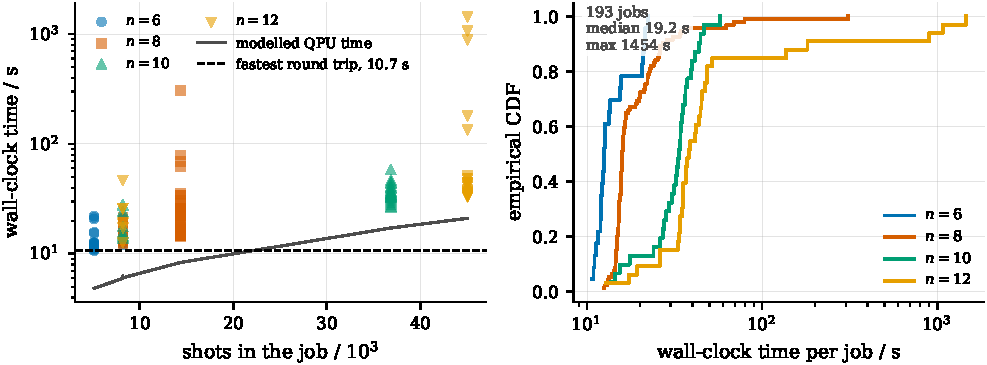
\includegraphics[width=\textwidth]{fig_cost.pdf}
\caption{The cost of a job on \ibmfez, from the \alljobs\ jobs of this study. \textbf{Left:}
measured wall-clock time from submission to result against the number of shots the job carried.
The dashed line is the fastest round trip observed, \minwall\,s; no job returned faster,
whatever it contained. \textbf{Right:} the empirical distribution of the same times, by
instance size. Both panels are measured; the modelled metered time of Eq.~\eqref{eq:cost} is
shown for scale only.}
\label{fig:cost}
\end{figure*}

The consequence for a variational loop is the same under either accounting. An optimizer that
submits one job per function evaluation pays the per-job overhead --- of order three seconds
metered, of order ten to twenty seconds in wall clock --- once per evaluation, before a single
shot is taken. A batched iteration that puts $M$ parameter vectors into one PUB pays it once
for all $M$. At the settings used below $M$ ranges from $10$ to $22$, so the serial arm spends
between $10$ and $22$ times as much per-job overhead for the same number of landscape points
examined. Table~\ref{tab:ledger} gives the full ledger.

Two scope limits belong here rather than in the discussion. First, wall-clock time is not a
property of the device or of the algorithm: it depends on other users' load and on fair-share
priority, and our own per-run ratios vary by a factor of four. It should be read as a
characterisation of the access mode, not as a constant. Second, and more important, that access
mode is job mode on the free tier. IBM's \texttt{Batch} and \texttt{Session} modes exist
precisely to amortise queueing across a sequence of jobs, and a user with access to them would
see a much smaller wall-clock penalty --- though the per-job metered overhead of
Eq.~\eqref{eq:cost} is charged in all three modes, and in \texttt{Session} mode the meter runs
on elapsed time whether or not a circuit is executing~\cite{ibmdocs_runtime}. The argument of
this paper is therefore strongest for the open-plan user and weakest for the reserved-capacity
one; it does not vanish for either.

\begin{table*}[t]
\caption{Resource ledger for the four main runs. ``QPU'' is Eq.~\eqref{eq:cost} evaluated on
each job's contents --- modelled, not measured, for the reason given in the text --- while
``wall'' is the measured sum of submission-to-result times. The two follow-up studies added
\oosjobs\ further jobs, giving \alljobs\ jobs for the study as a whole. Every job identifier is
in the released data.}
\label{tab:ledger}
\begin{ruledtabular}
\begin{tabular}{cccccccccc}
$n$ & $p$ & shots/cand. & shots/job & jobs & total shots & QPU\,/\,s
 & wall\,/\,s & ratio & median wall\,/\,s \\
\hline
6 & 2 & 512 & 5{,}120 & 20 & 111{,}600 & 100 & 292 & 2.9 & 13 \\
8 & 3 & 1024 & 14{,}336 & 24 & 325{,}612 & 193 & 942 & 4.9 & 23 \\
10 & 4 & 2048 & 36{,}864 & 28 & 946{,}160 & 448 & 968 & 2.2 & 34 \\
12 & 5 & 2048 & 45{,}056 & 30 & 1{,}241{,}066 & 587 & 4688 & 8.0 & 38 \\
\hline
total & & & & 102 & 2{,}624{,}438 & 1329 & 6890 & 5.2 & \\
\end{tabular}
\end{ruledtabular}
\end{table*}

% ======================================================================
\section{Batched pattern search}
\label{sec:optimizer}
% ======================================================================

Pattern search, also called compass or direct search, replaces derivatives with a fixed
stencil of trial points around an incumbent, accepting a move only when a trial point
improves on the incumbent and contracting the stencil when none does
\cite{torczon1997convergence,kolda2003directsearch}. Its relevant property here is
structural rather than statistical: the entire iteration is determined by the incumbent and
the current radius, so every point can be named before any value comes back.

Algorithm~1 states the variant used. For $2p$ parameters an iteration consists of
the incumbent (row $0$), the $2\times 2p$ axial probes at radius $\rho$, and, when the
previous iteration moved, one momentum probe continuing along the accepted step: at most
$4p+2$ points, all submitted as the rows of a single PUB in a single job.

\begin{figure}[t]
\vspace{2pt}\hrule\vspace{3pt}
\noindent\textbf{Algorithm 1.}~Batched pattern search. One iteration $=$ one job.
\vspace{2pt}\hrule\vspace{4pt}
\begin{algorithmic}[1]
\Require incumbent $\mathbf x_0$, radius $\rho$, shot budget $S_{\rm job}$ per job
\State $\mathbf x \gets \mathbf x_0$, \; $\mathbf x_{\rm prev} \gets \mathbf x_0$
\For{$j = 1 \dots J$} \Comment{$J$ = the job budget}
  \State $\mathcal{C} \gets \{\mathbf x\} \cup
         \{\mathbf x \pm \rho\,\mathbf e_i\}_{i=1}^{2p}$
  \If{$\mathbf x \neq \mathbf x_{\rm prev}$}
     \State $\mathcal{C} \gets \mathcal{C} \cup
            \{2\mathbf x - \mathbf x_{\rm prev}\}$ \Comment{momentum probe}
  \EndIf
  \State submit \textbf{one job}: one PUB, $|\mathcal{C}|$ parameter rows,
         $S_{\rm job}/|\mathcal{C}|$ shots each
  \State $v_c \gets \CVaR_\alpha$ of the distribution measured for $c\in\mathcal{C}$
  \State $\sigma \gets$ standard deviation of $\tilde H$ under row $0$
  \State $\epsilon \gets \tfrac12\,\sigma/\sqrt{S_{\rm job}/|\mathcal{C}|}$
         \Comment{shot-noise tolerance}
  \State $c^\star \gets \arg\min_{c} v_c$
  \If{$c^\star \neq \mathbf x$ \textbf{ and } $v_{c^\star} < v_{\mathbf x} - \epsilon$}
     \State $\mathbf x_{\rm prev} \gets \mathbf x$, \;
            $\mathbf x \gets c^\star$, \;
            $\rho \gets \min(1.3\rho, \pi/2)$
  \Else
     \State $\rho \gets \max(0.6\rho, 0.02)$
  \EndIf
\EndFor
\end{algorithmic}
\vspace{2pt}\hrule\vspace{2pt}
\end{figure}

Two details are not decoration. The acceptance test requires an improvement larger than
$\epsilon$, half the standard error of the measured energy of the incumbent row. Without it,
at the shot counts used here, the incumbent moves on nearly every iteration and the search
chases shot noise rather than the landscape; the same measurement that supplies the incumbent
value supplies $\sigma$, so the tolerance costs nothing. The momentum probe exploits the fact
that the batch has a spare row whenever the previous iteration moved, and extrapolates along
the accepted direction; it is the cheapest available approximation to a line search.

Because the number of candidates and the shots per job are both fixed in advance, the entire
quantum cost of a run of $J$ iterations is known before it starts, to the millisecond, from
Eq.~\eqref{eq:cost}. That is a practical property no serial optimizer has: COBYLA's
evaluation count is data-dependent and must be truncated at an arbitrary point.

The initial point is the linear ramp $\beta_k = \Delta t\,(1 - (k-\tfrac12)/p)$,
$\gamma_k = -\Delta t\,k/p$ with $\Delta t = 0.5$, an adiabatically motivated schedule of the kind
introduced in Ref.~\cite{zhou2020qaoa} and shown to avoid the local minima that plague random
initialization~\cite{sack2021annealinginit}; warm-starting from a classical relaxation is a
further option we did not use~\cite{egger2021warmstart}. The sign of $\gamma$ follows the convention of
Eq.~\eqref{eq:ising}.

% ======================================================================
\section{Protocol and controls}
\label{sec:protocol}
% ======================================================================

Each instance is run as a self-contained experiment with two arms under an identical budget.

\emph{Matched budget.} Both arms receive the same number of jobs $J$ and the same shots per
job $S_{\rm job}$. The batched arm spends a job on $M = 4p+2$ parameter vectors at
$S_{\rm job}/M$ shots each; the serial arm spends a job on one parameter vector at the whole
$S_{\rm job}$. The two arms therefore consume identical quantum resources by both metrics, and the
difference under test is the allocation.

We should be careful about how much this constraint costs the batched arm. Nominally it hands
the serial arm a $M$-fold advantage in shot noise per evaluation. In practice the pre-registered
tuning study of Appendix~\ref{app:tuning} found final quality flat in shots per candidate between
$512$ and $2048$, so a serial evaluation at $14\,336$ or $45\,056$ shots is far into the regime
where extra shots buy nothing, and the surplus cannot be spent anywhere else. The honest reading
is therefore that the shot-matching constraint is close to a nullity for the serial arm and the
comparison reduces to $M$ points per job against one. We keep it because it forecloses the
objection, not because it is a meaningful handicap.

One asymmetry runs the other way and should also be named. The batched arm's $M$ rows execute
inside a single job under one calibration snapshot, so comparisons among them are drift-free;
COBYLA's successive evaluations sit in different jobs, minutes apart, and carry inter-job drift
on top of shot noise. That is a real advantage of batching, and it is part of what the method
buys, but it means ``the only difference is the allocation'' would be too strong a statement.

\emph{The serial optimizer.} COBYLA~\cite{powell1994cobyla} with $\rho_{\rm beg}$ equal to the
pattern-search radius. It was chosen because it was the strongest of COBYLA, SPSA, Nelder--Mead
and Powell in the pre-registration study of Appendix~\ref{app:tuning} at every size, over the
range of job budgets used here; the control should be the best available serial method, not a
straw man. (SPSA is stronger at a budget of two jobs, and Powell overtakes beyond about forty
jobs; neither is the regime studied.) This is
consistent with published comparisons of optimizers under
noise~\cite{lavrijsen2020optimizers,bonetmonroig2023comparison}.

\emph{Error suppression.} Dynamical decoupling~\cite{viola1999decoupling,ezzell2023dd} on
idle qubits and Pauli twirling of gates and measurements~\cite{wallman2016twirling} were
enabled for every job; neither consumes extra shots. No zero-noise extrapolation or probabilistic error
cancellation~\cite{temme2017mitigation} was used, so the measured distributions are raw device
output apart from these two settings; the only mitigation applied anywhere in this paper is
post-selection on Hamming weight, which is free.

\emph{The $\gamma=0$ control.} After the optimization arms, one job is submitted at the
batched arm's best $\boldsymbol\beta$ with $\boldsymbol\gamma$ set to zero. The circuit has
\emph{identical} gate count and depth, but its ideal output is exactly $\ket{+}^{\otimes n}$.
Any structure that survives in it is the device's noise floor and not something the algorithm
found. This is the reference against which every claim below should be read.

\emph{The drift control.} The two arms necessarily run one after the other, so a device that
drifts over the half hour would flatter whichever arm ran in better conditions. The last job
of every run repeats the \emph{first} batched iteration verbatim. The mean shift in $\CVaR$
across the run was \driftsix, \drifteight, \driftten\ and \drifttwelve\ for
$n=6,8,10,12$ --- of the order of the shot noise, and of both signs, so no drift correction
is applied.

\emph{Two views of quality.} Because $n \le 12$, the noiseless output distribution of any
parameter vector is computable exactly and cheaply. We therefore report, alongside what the
device measured, an oracle curve: the exact noiseless approximation ratio, evaluated
classically, of the best point each arm holds after each job. For the batched arm ``holds''
means the \emph{incumbent} --- the point that has survived the acceptance test of
Algorithm~1 --- and the curve is the running maximum of that incumbent's noiseless ratio over
jobs. For the serial arm it is the running maximum over the points COBYLA has evaluated, which
is what COBYLA returns. Two things about this metric must be stated. It is deliberately
generous to the serial arm, since the batched arm is credited only with points its acceptance
rule kept, while COBYLA is credited with the best of everything it touched. And it is an oracle:
neither optimizer can compute it, and neither could at a size worth solving. It is a diagnostic
of the search, not a quantity either method returns, and it is why the study stops at $12$
qubits. The device read-outs of Sec.~\ref{sec:results} are the non-oracle counterpart.

\emph{Pre-registration.} Every hyperparameter --- $p$, shots, jobs, $\alpha$, the initial
radius, the penalty $\mu$ --- was fixed on a noise model of \ibmfez\ before any quantum
processing time was spent (Appendix~\ref{app:tuning}). The depth $p$ was subsequently raised
by hand for the larger instances; the consequences are discussed in
Sec.~\ref{sec:discussion}.

% ======================================================================
\section{Results}
\label{sec:results}
% ======================================================================

\subsection{Convergence per job}

Figure~\ref{fig:convergence} is the central result, and Table~\ref{tab:convergence}
quantifies it. The upper row shows the exact noiseless approximation ratio of each arm's
incumbent as a function of the number of jobs spent; the lower row shows what the device
reported.

\begin{figure*}[t]
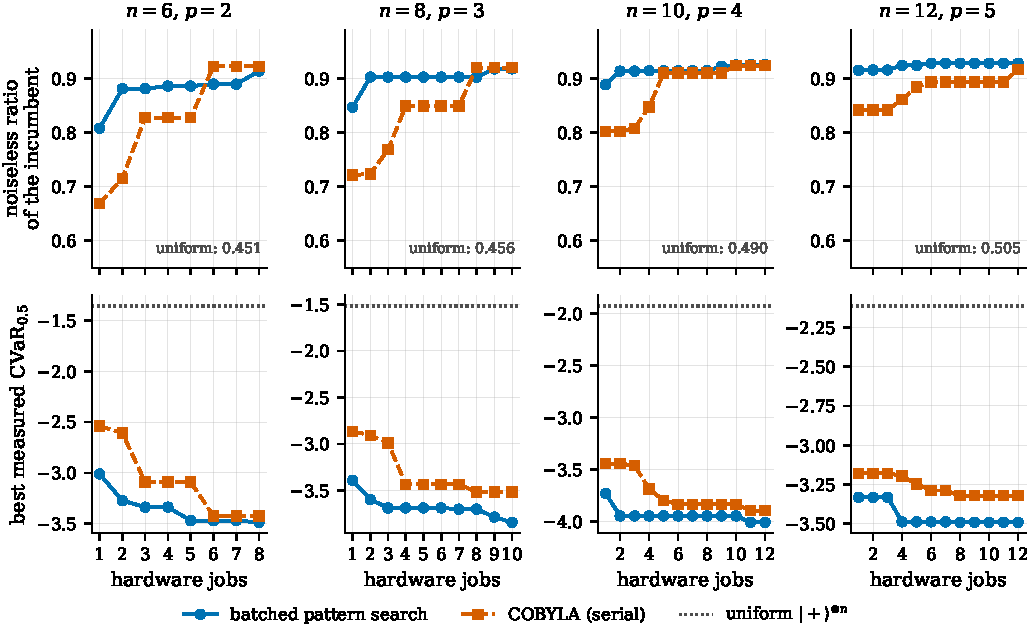
\includegraphics[width=\textwidth]{fig_convergence.pdf}
\caption{Optimization on \ibmfez\ under a matched budget of jobs and shots. \textbf{Upper:}
exact noiseless approximation ratio of the incumbent parameters, recomputed classically after
every job --- the quality of the point the optimizer has found, independent of how well the
device can realize it. \textbf{Lower:} best $\CVaR_{0.5}$ actually measured on the device.
Both arms receive the same number of jobs and the same shots per job; the batched arm spends a
job on $4p+2$ parameter vectors, the serial arm on one.}
\label{fig:convergence}
\end{figure*}

\begin{table*}[t]
\caption{Job efficiency on hardware. ``COBYLA needs'' is the number of jobs after which the
serial arm first reaches the quality the batched arm had after its \emph{first} job. ``Jobs to
95\%'' is the number of jobs each arm needs to reach $95\%$ of its own final noiseless ratio.}
\label{tab:convergence}
\begin{ruledtabular}
\begin{tabular}{ccccccccc}
& & & \multicolumn{2}{c}{after one BPS job} & \multicolumn{2}{c}{jobs to 95\%}
 & \multicolumn{2}{c}{best so far} \\
$n$ & $p$ & jobs/arm & $r_{\rm BPS}$ & COBYLA needs & BPS & COBYLA
 & $r_{\rm BPS}$ & $r_{\rm COB}$ \\
\hline
6 & 2 & 8 & 0.808 & 3 & 2 & 6 & 0.913 & 0.922 \\
8 & 3 & 10 & 0.847 & 4 & 2 & 8 & 0.918 & 0.920 \\
10 & 4 & 12 & 0.888 & 5 & 1 & 5 & 0.926 & 0.923 \\
12 & 5 & 12 & 0.915 & 12 & 1 & 5 & 0.928 & 0.916 \\
\end{tabular}
\end{ruledtabular}
\end{table*}

The pattern is consistent across all four instances, and the number of jobs COBYLA needs
to catch up grows along the sequence. We are cautious about reading that growth as a
size effect: the batch width $M = 4p+2$ and COBYLA's initial-model cost $2p+1$ both grow with
$p$, and $p$ was raised alongside $n$, so instance size and batch width are confounded here. The
claim we make is the weaker and safer one --- the ordering holds at every size tested, and at
$n=8$ it survives four independent initializations (Sec.~\ref{sec:replicates}). After a single
job the batched search is already at a noiseless ratio of \bpsjobonesix, \bpsjoboneeight,
\bpsjoboneten\ and \bpsjobonetwelve\ for $n=6,8,10,12$ --- a quality the serial arm first
matches only at job \jmatchsix, \jmatcheight, \jmatchten\ and \jmatchtwelve\ respectively.
Measured by the jobs each arm needs to reach $95\%$ of its own final value, the batched search
takes one or two and COBYLA five to eight. At $n=10$ the serial arm reaches the batched arm's one-job quality only at job~5, and at
$n=12$ only at the last job of its budget. The parameters each arm actually \emph{returns} for
the deep read-out --- not the same thing as the best point it ever touched --- are worth
\ratioidealbpsten\ against \ratioidealserten\ at $n=10$ and \ratioidealbpstwelve\ against
\ratioidealsertwelve\ at $n=12$ (Table~\ref{tab:final}).

The mechanism is visible in the lower row of Fig.~\ref{fig:convergence}. The serial traces
are jagged: COBYLA spends its early jobs building a linear model from single points, and
several of those points are worse than where it started. The batched traces are close to
monotone, because each job contains its own incumbent and a stencil around it, and the
acceptance test rejects moves that are not larger than shot noise. The batched arm is not
finding better optima --- at $n=6$ and $8$ the two arms end within $0.01$ of each other --- it
is finding them sooner --- one or two jobs against five to eight to reach $95\%$ of its own
plateau --- and that is precisely the currency that Sec.~\ref{sec:cost} shows to
be scarce.

\subsection{What the device delivered}

Figure~\ref{fig:final} and Table~\ref{tab:final} report the deep read-out at each arm's best
parameters, against the $\gamma=0$ control and the uniform baseline.

\begin{figure*}[t]
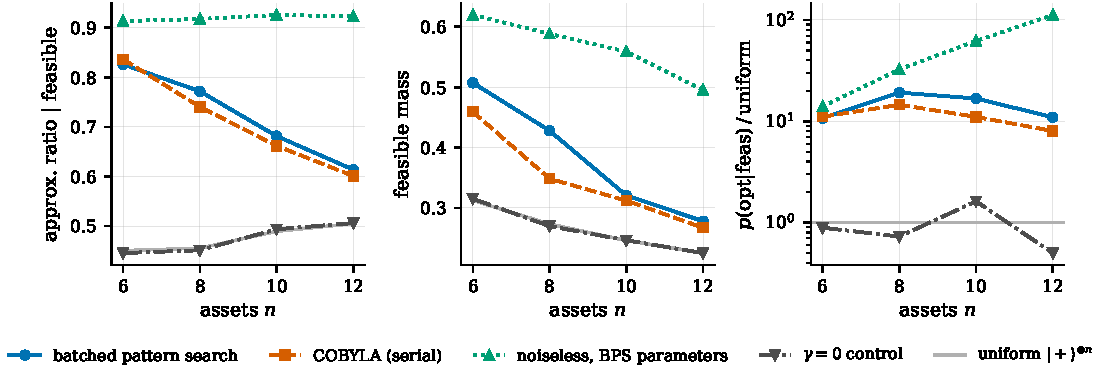
\includegraphics[width=\textwidth]{fig_final.pdf}
\caption{Final read-out quality against instance size, at $8192$ shots. The $\gamma=0$ control
runs a circuit of identical gate count and depth whose ideal output is $\ket{+}^{\otimes n}$;
it tracks the uniform baseline at every size, which is what licenses reading the separation
between the measured curves and that baseline as signal. The right panel is on a logarithmic scale; the downward
arrow on the $\gamma=0$ control at $n=12$ marks an upper bound, that circuit having never
sampled the optimum in $8192$ shots.}
\label{fig:final}
\end{figure*}

\begin{table*}[t]
\caption{Final read-out on \ibmfez. $\rho_s$ is the Spearman rank correlation between the
measured probability of a feasible portfolio and its exact cost; $\rho_s^{\gamma=0}$ is the
same quantity for the noise-floor control.}
\label{tab:final}
\begin{ruledtabular}
\begin{tabular}{ccccccccccc}
& \multicolumn{4}{c}{approximation ratio $\mid$ feasible}
 & \multicolumn{2}{c}{feasible mass} & & & \multicolumn{2}{c}{rank corr.} \\
$n$ & BPS & COBYLA & $\gamma{=}0$ & uniform & BPS & uniform
 & $\frac{p({\rm opt}\mid{\rm feas})}{\rm uniform}$ & rank of opt.
 & $\rho_s$ & $\rho_s^{\gamma=0}$ \\
\hline
6 & 0.826 & 0.836 & 0.446 & 0.451 & 0.507 & 0.312 & 10.7 & 1/20 & $-0.97$ & $+0.07$ \\
8 & 0.772 & 0.740 & 0.451 & 0.456 & 0.428 & 0.273 & 19.2 & 1/70 & $-0.88$ & $+0.07$ \\
10 & 0.681 & 0.662 & 0.494 & 0.490 & 0.321 & 0.246 & 16.8 & 1/252 & $-0.74$ & $-0.08$ \\
12 & 0.614 & 0.601 & 0.506 & 0.505 & 0.278 & 0.226 & 11.0 & 2/924 & $-0.45$ & $-0.00$ \\
\end{tabular}
\end{ruledtabular}
\end{table*}

Three observations. First, the device output is well separated from its own noise floor at
every size: the batched arm reaches a conditional approximation ratio of \ratiosix,
\ratioeight, \ratioten\ and \ratiotwelve\ against a $\gamma=0$ control at \ratioctrlsix,
\ratioctrleight, \ratioctrlten\ and \ratioctrltwelve, the latter tracking the uniform
baseline to within $0.005$ in every case. Second, the batched arm's read-out is better than
the serial arm's at $n=8$, $10$ and $12$ and marginally worse at $n=6$. At $n=10$ and $12$ this
tracks the noiseless quality of the returned parameters (\ratioidealbpsten\ against
\ratioidealserten, \ratioidealbpstwelve\ against \ratioidealsertwelve); at $n=6$ and $8$ the two parameter sets are
noiselessly equivalent to within $0.01$, so the measured difference there reflects device noise
rather than a property of the optimizer and should not be read as one --- which is what the
replicate study of Sec.~\ref{sec:replicates} is for. Third, and most directly relevant to a
user, the probability of sampling the exact optimum conditioned on feasibility is enhanced
over uniform by factors of \enhsix, \enheight, \enhten\ and \enhtwelve.

The separation from the baseline narrows as $n$ grows, from $0.38$ at $n=6$ to $0.11$ at
$n=12$. Section~\ref{sec:noise} shows why, and Sec.~\ref{sec:discussion} argues that a
substantial part of the narrowing is a consequence of the circuit depth having been increased
along with the instance size, not of the instance size alone.

\subsection{The device ranks portfolios}

A user of a portfolio optimizer does not need the exact minimizer; they need a short list.
Figure~\ref{fig:ranking} plots, for every feasible portfolio, the probability the device
assigned it against its exact cost.

\begin{figure*}[t]
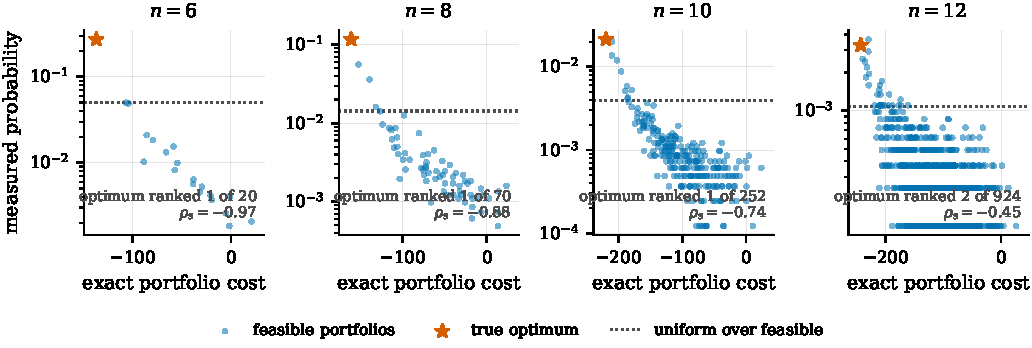
\includegraphics[width=\textwidth]{fig_ranking.pdf}
\caption{Measured probability of every feasible portfolio against its exact cost, from the
batched arm's read-out. The star is the true optimum; $\rho_s$ is the Spearman rank
correlation. The corresponding correlation for the $\gamma=0$ control is
$\rho_s^{\gamma=0} = \rhoctrlsix, \rhoctrleight, \rhoctrlten, \rhoctrltwelve$ for
$n=6,8,10,12$ --- consistent with zero.}
\label{fig:ranking}
\end{figure*}

The relationship is monotone and strong: $\rho_s = \rhosix$, \rhoeight, \rhoten\ and
\rhotwelve. The true optimum is the \emph{most probable} feasible outcome at $n=6$, $8$ and
$10$, and the second most probable of \nfeastwelve\ candidates at $n=12$. The same statistic
computed on the $\gamma=0$ control is consistent with zero at every size
($|\rho_s^{\gamma=0}| \le 0.08$), which is the check that makes the correlation meaningful:
a circuit of the same depth on the same qubits, differing only in that its cost-layer angles
are zero, carries no information about the cost function whatsoever. Whatever the device is
doing at $n=12$, it is not sorting portfolios by an artefact of the readout chain or the
gate set.

\subsection{The device as a depolarizing channel}
\label{sec:noise}

The measured distributions are well described by a single-parameter model. Writing $P_{\rm
ideal}$ for the exact QAOA distribution at the measured parameters, we fit
\begin{equation}
  P_{\rm dev} \;=\; \mathcal{R}\Big[(1-\eta)P_{\rm ideal} + \eta\,\mathcal{U}\Big] ,
  \label{eq:twin}
\end{equation}
where $\mathcal{U}$ is uniform and $\mathcal{R}$ applies independent readout bit flips at the
measured rate, choosing $\eta$ so that the model reproduces the measured mean energy --- one
fitted number per instance. The resulting $\eta$ are \etasix, \etaeight, \etaten\ and
\etatwelve\ at $\Ntwoq = \ntwoqsix$, \ntwoqeight, \ntwoqten\ and \ntwoqtwelve\ two-qubit
gates.

\begin{figure*}[t]
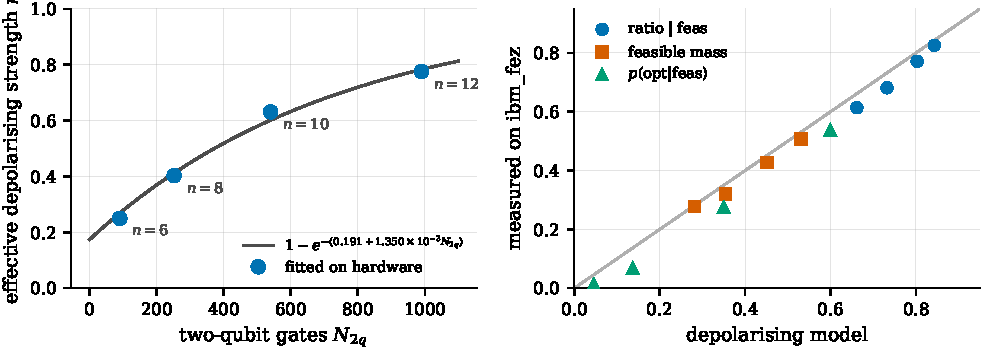
\includegraphics[width=\textwidth]{fig_noise.pdf}
\caption{\textbf{Left:} effective depolarizing strength $\eta$ fitted to the measured mean
energy of each instance, against the two-qubit gate count of its circuit; the line is
Eq.~\eqref{eq:etalaw}, a two-parameter fit to the four points. \textbf{Right:} the model of
Eq.~\eqref{eq:twin}, with $\eta$ fitted only to the mean energy, against the measured values
of three quantities it was not fitted to.}
\label{fig:noise}
\end{figure*}

These four numbers are described by
\begin{equation}
  \eta(\Ntwoq) \;=\; 1 - \exp\!\big[-(\etaa + \etab\times 10^{-3}\,\Ntwoq)\big]
  \label{eq:etalaw}
\end{equation}
to within \etamaxres\ (Fig.~\ref{fig:noise}, left). The slope corresponds to an effective
error of $1.35\times10^{-3}$ per two-qubit gate, about half the median CZ error of
\czerr\% reported by the device calibration, which is the expected relationship: a
depolarizing channel acting on the \emph{output distribution} is a weaker statement than one
acting on the state, and Pauli twirling makes the coherent part of the error stochastic and
therefore partially benign. The intercept, $\etaa$, is the depth-independent contribution ---
state preparation, single-qubit gates and measurement.

The right panel of Fig.~\ref{fig:noise} tests the model against quantities it was not fitted
to. It reproduces the conditional approximation ratio to within \twinratiodev\ and the feasible
mass to within \twinfeasdev\ at every size, and under-predicts the loss in
$p(\text{optimum}\mid\text{feasible})$,
which is expected: a global depolarizing channel damages the whole distribution uniformly,
whereas correlated and coherent errors damage the sharp peak disproportionately. Equation
\eqref{eq:etalaw} is therefore useful as a resource-planning tool --- it converts a proposed
$(n,p)$ into a predicted output quality before any time is spent --- and mildly optimistic as
a physical description.

\subsection{Depth is a trade-off, and its optimum is shallow}
\label{sec:depth}

The circuit depth was increased along with the instance size in the runs above, which leaves the
two effects entangled. They can be separated without an optimizer at all. For $n \le 12$ the
noiseless QAOA landscape can be optimized \emph{exactly and classically}, so for each $(n,p)$ we
computed the best parameters any optimizer could ever return at that depth, and then simply
measured what the device made of them: one job, $8192$ shots, \depthjobs\ jobs in total for
$4$ sizes $\times\ 5$ depths plus a second parameter set at $n=12$, costing \depthqpu\,s of
metered time. The optimizer is removed from
the picture and only the depth--noise trade-off remains.

\begin{figure*}[t]
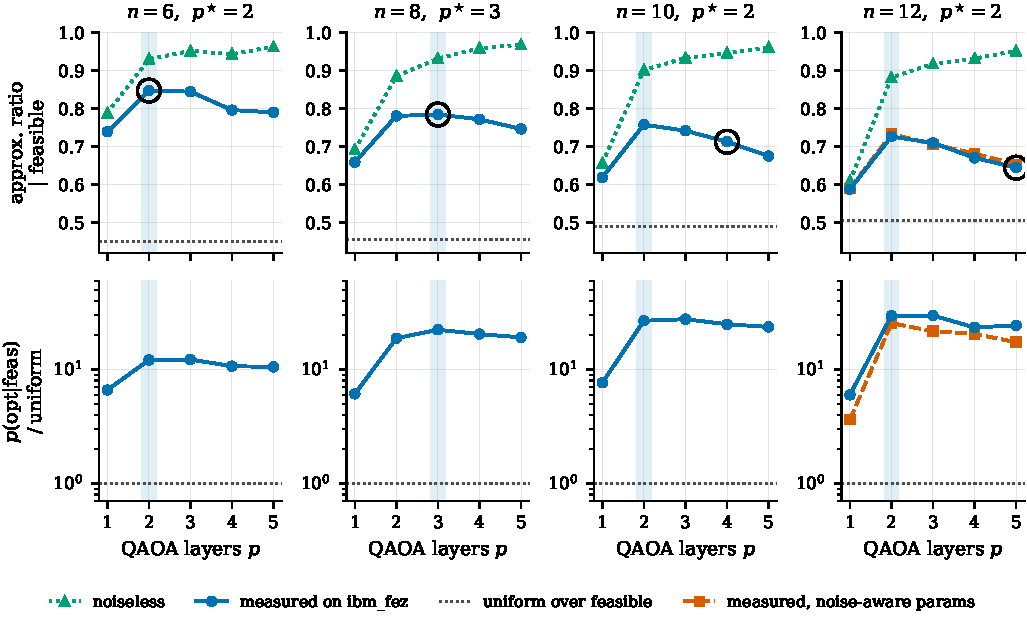
\includegraphics[width=\textwidth]{fig_depth.pdf}
\caption{Approximation ratio against circuit depth at \emph{classically optimal} parameters. The
noiseless curve (green) rises with $p$; the measured curve (blue) rises, peaks at
$p^\star$ (shaded), and falls, because $3p\binom{n}{2}$ two-qubit gates eventually cost more
fidelity than an extra layer buys. Black rings mark the depth actually used for that size in
Sec.~\ref{sec:results}. At $n=12$ the orange curve repeats the measurement at parameters
optimized against the noise model of Eq.~\eqref{eq:twin} instead of the noiseless landscape.
\textbf{Lower:} the probability of sampling the exact optimum, conditioned on feasibility, as a
multiple of the uniform value $1/\binom{n}{B}$; it peaks at the same depth.}
\label{fig:depth}
\end{figure*}

\begin{table}[t]
\caption{Depth scan on \ibmfez, $8192$ shots per point, at classically optimal parameters.
First row of each triple: measured approximation ratio. Second, in italic: the exact noiseless
value at the same parameters. Third: the measured $p(\text{optimum}\mid\text{feasible})$ as a
multiple of the uniform value $1/\binom{n}{B}$.}
\label{tab:depth}
\begin{ruledtabular}
\begin{tabular}{cccccccc}
$n$ & $p=1$ & $p=2$ & $p=3$ & $p=4$ & $p=5$ & $p^\star$ & $p$ run \\
\hline
6 & 0.739 & 0.847 & 0.845 & 0.796 & 0.790 & 2 & 2 \\
& \textit{0.788} & \textit{0.930} & \textit{0.952} & \textit{0.943} & \textit{0.963} & & \\
& \small{7$\times$} & \small{12$\times$} & \small{12$\times$} & \small{11$\times$} & \small{11$\times$} & & \\[3pt]
8 & 0.659 & 0.781 & 0.784 & 0.772 & 0.747 & 3 & 3 \\
& \textit{0.692} & \textit{0.885} & \textit{0.932} & \textit{0.959} & \textit{0.968} & & \\
& \small{6$\times$} & \small{19$\times$} & \small{22$\times$} & \small{20$\times$} & \small{19$\times$} & & \\[3pt]
10 & 0.619 & 0.758 & 0.742 & 0.713 & 0.675 & 2 & 4 \\
& \textit{0.657} & \textit{0.902} & \textit{0.933} & \textit{0.946} & \textit{0.961} & & \\
& \small{8$\times$} & \small{27$\times$} & \small{28$\times$} & \small{25$\times$} & \small{24$\times$} & & \\[3pt]
12 & 0.588 & 0.727 & 0.710 & 0.671 & 0.645 & 2 & 5 \\
& \textit{0.609} & \textit{0.882} & \textit{0.918} & \textit{0.932} & \textit{0.952} & & \\
& \small{6$\times$} & \small{30$\times$} & \small{30$\times$} & \small{23$\times$} & \small{24$\times$} & & \\[3pt]
\end{tabular}
\end{ruledtabular}
\end{table}

Figure~\ref{fig:depth} and Table~\ref{tab:depth} show the expected shape, now measured rather
than argued. The noiseless ratio rises with $p$ at every size, reaching $0.95$--$0.97$ by $p=5$;
it is monotone at $n=8$, $10$ and $12$, and at $n=6$ dips by $0.009$ between $p=3$ and $p=4$,
which is the multi-start classical optimizer failing to find the global optimum of a
$8$-parameter landscape rather than anything physical. The measured ratio does not: it rises steeply from $p=1$, peaks, and then declines. The
peak sits at $p^\star = \pstarsix, \pstareight, \pstarten, \pstartwelve$ for
$n = 6, 8, 10, 12$, but these are single $8192$-shot jobs and at $n=6$ and $n=8$ the top two
depths differ by only $0.002$ and $0.003$, which is within shot noise; the statement the data
support is that the optimum lies at $p = 2$ or $3$ at every size, not which of the two. At $n=12$ the measured value falls from \depthbesttwelve\ at $p=2$ to
\depthruntwelve\ at $p=5$ even though the noiseless value has risen from $0.882$ to $0.952$ over
the same range.

This settles the confound of Sec.~\ref{sec:results} and is worth stating plainly. The depths run
in the main study were $p = 2, 3, 4, 5$; the measured optima are $2, 3, 2, 2$. The $n=6$ and $n=8$
runs were therefore \emph{at} the device optimum, while the $n=10$ and $n=12$ runs were past it,
by \depthgaintwelve\ in approximation ratio at $n=12$. Part of the decline across
Fig.~\ref{fig:final} is thus a depth artefact rather than a property of the instance --- though
not all of it: even at each size's own optimal depth the measured ratio still falls with $n$,
from \depthbestsix\ through \depthbesteight\ and \depthbestten\ to \depthbesttwelve.

The second measurement at $n=12$ answers the obvious follow-up. If the loss comes from running
too deep, could an optimizer that \emph{knew} about the noise recover it by choosing different
parameters at the same depth? We reoptimized against the model of Eq.~\eqref{eq:twin} at the
$\eta$ predicted by Eq.~\eqref{eq:etalaw} and measured the result. It changes nothing: the
noise-aware parameters differ from the noiseless-optimal ones by at most \noiseawaremax\ in
measured ratio, in either direction, at every depth (orange curve, Fig.~\ref{fig:depth}). The
depth is the ceiling, not the parameter choice --- consistent with the picture in which the dominant
error is a global depolarizing channel, which contracts the whole output distribution toward
the uniform one and therefore cannot be steered around by a change of parameters. That noisy
devices are limited in exactly this way, and that the limitation tightens with circuit volume,
is the subject of a body of rigorous
work~\cite{stilckfranca2021limitations,wang2021noisebp} which our measurement is a small
concrete instance of.

The practical rule this yields is concrete: at a given device error rate, choose $p$ by
maximizing the product of the noiseless ratio and $1-\eta(3p\binom{n}{2})$ from
Eq.~\eqref{eq:etalaw}, which for \ibmfez\ at these sizes lands on $p = 2$ or $3$ and is
computable before a single job is submitted.

\subsection{Repeatability across initializations}
\label{sec:replicates}

The comparison of Sec.~\ref{sec:results} is one trajectory per arm per size. To attach a spread to
it we repeated the $8$-asset experiment from three further starting points, changing nothing else:
same instance, same $p=3$, same shots, same ten jobs per arm, same $14\,336$ shots per job for both
arms. The starts are the linear ramp at $\Delta t \in \{0.35, 0.50, 0.60, 0.85\}$, with
$\Delta t = 0.50$ the run already reported; within a start both arms receive the \emph{same}
initial point.

\begin{figure*}[t]
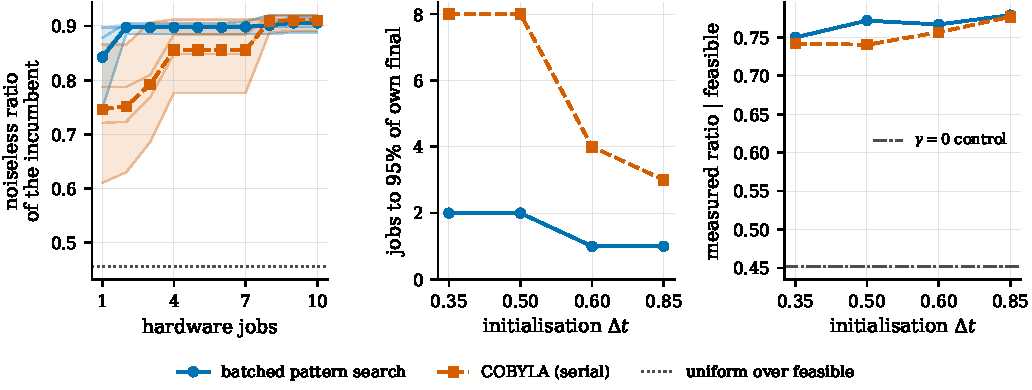
\includegraphics[width=\textwidth]{fig_replicates.pdf}
\caption{Four independent initializations at $n=8$, $p=3$. \textbf{Left:} noiseless approximation
ratio of the incumbent against jobs; thin lines are individual starts, markers the mean, bands the
full range. \textbf{Centre:} jobs each arm needed to reach $95\%$ of its own final value.
\textbf{Right:} measured approximation ratio of the deep read-out at each arm's returned
parameters, against the $\gamma=0$ noise floor.}
\label{fig:replicates}
\end{figure*}

\begin{table}[t]
\caption{The $8$-asset comparison from four initializations, \repjobs\ jobs and \repqpu\,s of
metered time. ``COBYLA matches at'' is the job at which the serial arm first reaches the quality
the batched arm had after its first job; ``final, noiseless'' is the exact quality of the returned
parameters and ``read-out'' the measured approximation ratio at those parameters.
$^{\dagger}$ is the run reported in Sec.~\ref{sec:results}.}
\label{tab:replicates}
\begin{ruledtabular}
\begin{tabular}{cccccccccc}
& \multicolumn{2}{c}{after one job} & COBYLA & \multicolumn{2}{c}{jobs to 95\%} & \multicolumn{2}{c}{best so far} & \multicolumn{2}{c}{read-out} \\
$\Delta t$ & BPS & COB & matches at & BPS & COB & BPS & COB & BPS & COB \\
\hline
0.35\phantom{$^\dagger$} & 0.748 & 0.611 & 4 & 2 & 8 & 0.888 & 0.891 & 0.750 & 0.742 \\
0.50$^{\dagger}$ & 0.847 & 0.721 & 4 & 2 & 8 & 0.918 & 0.920 & 0.772 & 0.740 \\
0.60\phantom{$^\dagger$} & 0.878 & 0.788 & 4 & 1 & 4 & 0.920 & 0.919 & 0.767 & 0.757 \\
0.85\phantom{$^\dagger$} & 0.897 & 0.866 & 3 & 1 & 3 & 0.898 & 0.912 & 0.779 & 0.777 \\
\hline
mean & 0.843 & 0.746 & & 1.50 & 5.75 & 0.906 & 0.910 & 0.767 & 0.754 \\
\end{tabular}
\end{ruledtabular}
\end{table}

The ordering holds at every start (Fig.~\ref{fig:replicates}, Table~\ref{tab:replicates}). The
batched search needs \repnbrange\ jobs to reach $95\%$ of its own final value, mean \repnbmean;
COBYLA needs \repnsrange, mean \repnsmean. After a single job the batched arm is at
\repbpsjobone\ on average against \repserjobone\ for the serial arm, and COBYLA first matches the
batched arm's one-job quality at job $3$, $4$, $4$ and $8$ across the four starts.

Two further features are worth noting. The \emph{final} parameter values are statistically
indistinguishable --- \repbpsfinal\ $\pm$ \repbpssd\ for the batched arm against \repserfinal\
$\pm$ \repsersd\ for the serial one --- which is the same message as Sec.~\ref{sec:results}: the
two methods find equally good parameters, and differ in how many round trips it takes. The deep
read-outs at those parameters (Fig.~\ref{fig:replicates}, right) tell the same story with a
slight edge to the batched arm: \repmeasbps\ $\pm$ \repmeasbpssd\ against \repmeasser\ $\pm$
\repmeassersd, with the batched arm ahead at \repwins\ of the four starts, and both far above the
$\gamma=0$ noise floor at \ratioctrleight. And the
advantage is largest where it matters most, at the poor starting point: at $\Delta t = 0.35$ the
batched arm is at $0.748$ after one job while the serial arm is at $0.611$ and needs eight jobs to
converge, whereas at $\Delta t = 0.85$, where the ramp already lands near a good region, both arms
converge quickly and the gap narrows to two jobs. A practitioner who cannot pre-tune their
initialization --- which is the situation whenever the instance is too large to simulate --- is
exactly the practitioner for whom the batched method buys the most.

% ======================================================================
\section{Discussion}
\label{sec:discussion}
% ======================================================================

\subsection{What the comparison does and does not show}

The batched search does not reliably find better optima than COBYLA. Measured by the best point
each arm reached, three of the four instances end within $0.01$; measured by the parameters each
arm actually returned, the two are level at $n=6$ and $8$ and the batched arm is ahead at $n=10$
and $12$. What it does is
find them in one or two jobs instead of five to eight, and Sec.~\ref{sec:cost} establishes
that jobs are what a cloud user actually spends. The claim is about the shape of the
convergence curve near the origin, not about its asymptote, and the practical regime it
speaks to is the one where a user has time for a handful of round trips rather than a hundred.

Several limitations bound the strength of the evidence, and we would rather name them than
have them found.

\emph{Replication.} The four main instances were each run once. The replicate study of
Sec.~\ref{sec:replicates} attaches a spread to the $8$-asset comparison --- \repnbmean\ jobs
against \repnsmean\ across four initializations, with the ordering holding at every one --- but
the $10$- and $12$-asset results are single trajectories, and the differences in \emph{final}
quality there ($0.043$ and $0.032$ in the returned parameters) should be read against the
replicate spread of $\pm 0.01$ rather than as precise.

\emph{Sequential arms.} The two arms ran one after the other rather than interleaved. The drift
control of Sec.~\ref{sec:protocol} is a single paired repeat per instance, which cannot separate
drift from shot noise; it bounds the effect at a few hundredths of a $\CVaR$ unit and no more
than that. Interleaving would have been cleaner and costs nothing.

\emph{Ablations we did not run.} Two would sharpen the attribution and each costs one job budget.
A \emph{random}-batch arm --- $M$ points per job drawn around the same start, greedily tracked
--- would separate the value of batching per se from the value of the pattern-search stencil. A
\emph{serial} pattern search, one point per job with the same acceptance rule, would separate the
stencil from the shot-noise tolerance of Algorithm~1, which is a noise-robustness property COBYLA
has no analogue of. As designed, this experiment measures the package, not its parts.

\emph{A batchable competitor.} COBYLA was chosen because it was the strongest \emph{serial}
method in the pre-registration study, but as Sec.~\ref{sec:intro-batching} notes, SPSA and
parameter-shift gradients are themselves batchable. A batched SPSA or a multistart COBYLA packing
several concurrent chains into one PUB is the harder target, and we did not run it.

\emph{The oracle metric.} The per-job curve of Fig.~\ref{fig:convergence} uses the exact
noiseless ratio, which no optimizer can compute and which does not exist at a problem size worth
solving. It diagnoses the search; it is not a quantity either method returns. The device
read-outs of Table~\ref{tab:final} and Table~\ref{tab:replicates} are the non-oracle
counterpart, and there the two arms are much closer.

\emph{Selection bias in the measured traces.} The lower row of Fig.~\ref{fig:convergence} plots
a running minimum of measured $\CVaR$. The batched arm takes that minimum over $M$ values per
job and the serial arm over one, so the batched trace carries a winner's-curse bias downward.
This is one reason the separation is much larger there than in the independently measured deep
read-outs, and the read-outs are the number to trust.

\subsection{Depth and instance size were varied together}

The circuit depth was increased with the instance size, $p = 2,3,4,5$ for $n = 6,8,10,12$, so the
decline in measured quality across Fig.~\ref{fig:final} confounds two effects. The depth scan of
Sec.~\ref{sec:depth} separates them by direct measurement: the device optimum sits at
$p^\star = \pstarsix, \pstareight, \pstarten, \pstartwelve$, so the $n = 6$ and $n = 8$ runs were
at that optimum and the $n = 10$ and $n = 12$ runs were beyond it. Part of the decline is therefore
a depth artefact --- worth \depthgaintwelve\ in approximation ratio at $n=12$ --- and part is
genuine, since the ratio at each size's own best depth still falls from \depthbestsix\ to
\depthbesttwelve\ as $n$ grows. Repeating the $n=12$ optimization at $p=2$ rather than $p=5$ is
the obvious next experiment; on the evidence of Table~\ref{tab:depth} it would raise the final
read-out substantially, and it would not change the job-efficiency comparison, which is a
statement about the optimizer at fixed circuit.

\subsection{Consequences beyond QAOA}

The cost model of Eq.~\eqref{eq:cost} is a property of the access mode, not of the algorithm.
Any variational procedure driven through a queue --- a chemistry eigensolver, a quantum
kernel evaluation, a circuit-parameter calibration, an error-mitigation sweep --- pays the
same fixed charge per round trip and can, in principle, fill the same PUB. Three consequences
seem general.

First, \emph{benchmark against a job budget}. Reporting convergence against function
evaluations makes a serial and a batched optimizer look comparable when their hardware costs
differ by an order of magnitude. A plot against submitted jobs is the honest one on cloud
hardware, and it is a different plot. The application-oriented benchmarking effort of
Ref.~\cite{lubinski2023benchmarks} already reports execution time including cloud overheads and
is the natural home for a job-count axis alongside it.

Second, \emph{prefer optimizers whose next batch is knowable}. This is a design criterion distinct
from sample efficiency, and it admits degrees. Pattern search names $4p+2$ points per round
trip; parameter-shift gradients~\cite{mitarai2018qcl,schuld2019gradients} name $4p$;
SPSA~\cite{spall1992spsa} and its quantum-natural variant~\cite{gacon2021qfi} name two; batched
Bayesian and information-sharing schemes~\cite{self2021infosharing} name as many as one chooses;
model-based trust-region methods~\cite{sung2020models} and multistart
schemes~\cite{shaydulin2019multistart} name a design set. COBYLA, Nelder--Mead and Powell name
one. A method that is slightly worse per evaluation but names $M$ points at a time can be an
order of magnitude better per job, and the classical direct-search literature worked out how to
exploit exactly this parallelism decades ago~\cite{hough2001apps}.

Third, \emph{state the cost model with the result}. The community reports shots because shots
were once the binding constraint. On queued hardware in 2026 they are frequently not, and a
paper that reports only shots leaves the reader unable to reconstruct what the experiment
would cost them.

We note also what the job-budget framing does \emph{not} rescue. Nothing here addresses the
fundamental obstacles to variational scaling --- barren plateaus~\cite{mcclean2018barren} and
their noise-induced counterpart~\cite{wang2021noisebp} --- and the narrowing separation
between the measured curves and the noise floor in Fig.~\ref{fig:final} is a reminder that
at $12$ qubits and $990$ two-qubit gates, $78\%$ of the output distribution is already
uniform. Job efficiency buys a shorter path to whatever the device can deliver; it does not
change what that is.

% ======================================================================
\section{Conclusion}
% ======================================================================

We measured what a job costs on a superconducting quantum processor and found a fixed charge of
$3.00\,$s of metered time --- a three-constant law that, once fitted, predicted a further
\oosjobs\ jobs on recalibrated hardware to within \oosres\,ms --- plus a wall-clock overhead that
made \allwallmin\ minutes of real time buy \allqpumin\ minutes of quantum processing. Under that cost model we compared a
batched pattern search, which spends one job on $4p+2$ points of the variational landscape,
against COBYLA, which spends one job on one point, at matched jobs and matched shots, on four
nested cardinality-constrained portfolio problems solved on \ibmfez\ and verified by
exhaustive enumeration. The batched search reached in a single job a parameter quality that
the serial optimizer required three to twelve jobs to match, with the gap widening as the
instance grew. The device returned the exact optimum as its most probable feasible outcome at
three of the four sizes and as its second most probable at the fourth, with rank correlations
against the exact ordering from $\rho_s = \rhosix$ to $\rho_s = \rhotwelve$, while an
identically deep $\gamma=0$ control showed no correlation at all. Two follow-up studies closed
the obvious gaps: repeating the $8$-asset comparison from four initializations left the ordering
intact at every one, and a depth scan at classically optimal parameters located the device's
optimal circuit depth at $p = 2$--$3$ and showed that reoptimizing against the noise model
recovers nothing beyond it.

The specific method is simple and, we would argue, is not the point. The point is the unit of
account. As long as quantum processors are reached through queues, the number of times an
algorithm goes around the loop is the cost that binds, and algorithms should be designed and
reported accordingly.

\begin{acknowledgments}
The author thanks IBM Quantum for access to \ibmfez. This work was carried out entirely within
the $180$ minutes of quantum processing time granted under the IBM Quantum Open Plan promotion
of March 2026, and used \totqpumin\ minutes for the four main runs and a further \oosqpu\,s for the two
follow-up studies, \allqpumin\ minutes in all. The author is a member of the Qiskit Advocate
Program. The views expressed are those of the author and do not reflect the official policy or
position of IBM or the IBM Quantum team.
\end{acknowledgments}

\section*{Data and code availability}

Every quantum result in this paper is reproduced by six self-contained Jupyter notebooks --- one
per instance size, plus the replicate and depth-scan studies --- released together with the raw
data they produced: the complete job log
including every IBM job identifier, the measured bitstring counts of every candidate of every
job, both optimization traces, the control read-outs and the final metrics. Figures and tables
are generated from those files by the included scripts, and every number quoted in the text is
emitted by the same scripts rather than transcribed. The archive is available at
\url{https://github.com/<user>/qaoa-job-budget} and archived at Zenodo,
DOI \texttt{<to be assigned>}; code is released under the MIT licence and data under
CC-BY-4.0.

\appendix

% ======================================================================
\section{Selecting the hyperparameters before spending hardware time}
\label{app:tuning}
% ======================================================================

Every hyperparameter was fixed on a noise model of \ibmfez\ before any quantum processing time
was spent. Full noisy simulation is too slow to sweep --- one $12$-qubit, $p=2$ circuit at
$2048$ shots costs about $80\,$s with a full Aer noise model --- so the sweep used the
one-parameter surrogate of Eq.~\eqref{eq:twin}, with $\eta$ fitted per $(n,p)$ against Aer at
two parameter points. The surrogate reproduced Aer's $\CVaR$ to about $0.1$ in normalized
units and its feasible mass to about $0.05$.

The sweep covered $p \in \{1,2,3\}$, shots per candidate $\in \{512, 1024, 2048\}$, jobs per
arm $\in \{8,12,16\}$, $\alpha \in \{0.1, 0.25, 0.5\}$ and initial radius $\in \{0.25, 0.4\}$,
filtered to configurations fitting a $300\,$s budget, at ten random seeds each --- $480$
configurations in total, and a further confirmation study at forty seeds. It selected
$\alpha = 0.5$ at every size, an initial radius of $0.25$, and found quality flat in shots
between $512$ and $2048$ and flat in jobs beyond about ten. On the surrogate, COBYLA needed sixteen jobs to match what the batched
search had after twelve at $n = 6$, $8$ and $10$, and did not match it within sixty-four at
$n = 12$; the hardware runs of Sec.~\ref{sec:results} reproduce that ordering, though the
surrogate carries neither crosstalk nor drift and its absolute numbers should not be compared
with the device's.

The surrogate selected $p=2$ at all four sizes, on the grounds that $p=3$ improved the
predicted ratio by at most $0.011$ for $50\%$ more two-qubit gates. The depths actually run were
$p = 2,3,4,5$, chosen by hand in the belief that a larger instance warrants a deeper circuit. The
hardware depth scan of Sec.~\ref{sec:depth} vindicated the surrogate: the measured optimum is
$p = 2$ or $3$ at every size. A fake backend carries no crosstalk and no drift, which is precisely
why the $\gamma=0$ and drift controls of Sec.~\ref{sec:protocol} are part of every hardware run;
but on the one question where its recommendation was overruled, it was right.

% ======================================================================
\section{Reproducing the experiment}
\label{app:repro}
% ======================================================================

Each notebook is self-contained and runs top to bottom against \ibmfez\ in roughly $100$ to
$600\,$s of metered time. A \texttt{DRY\_RUN} switch replaces the device with the surrogate of
Eq.~\eqref{eq:twin} and executes the entire experiment in about a minute at no cost, which is
the recommended first step. The ledger of Sec.~\ref{sec:cost} is enforced at run time: before
every submission the notebook predicts the metered cost from Eq.~\eqref{eq:cost}, switches
from the model to the device's own reported usage after two jobs, and refuses to submit a job
that would exceed the configured cap.

Three implementation details caused errors that are silent rather than loud, and are recorded
here because they would cost another user a run.
\begin{enumerate}
\item \texttt{BitArray.get\_int\_counts()} called with no argument merges the counts of
      \emph{all} parameter rows of a PUB into one dictionary. A batched run that does this
      produces plausible output and is entirely meaningless. The row index is mandatory.
\item The parameters of a transpiled circuit are ordered by \emph{name}, not by construction
      order. The array of parameter values must be assembled by name lookup.
\item An explicit \texttt{initial\_layout} must be asserted to have survived the pass manager;
      otherwise the circuit can silently move off the chosen chain.
\item Reading the runtime's reported usage through \texttt{job.metrics()} is version-dependent,
      and a \texttt{try/except} around it will hide a wrong key path behind a plausible fallback.
      Ours did, on every job of this study, which is why the metered times reported in
      Sec.~\ref{sec:cost} are modelled rather than measured. If you want the device's own number,
      assert that you got one.
\end{enumerate}

The first and the last of these have the same shape: a silent fallback that produces output
indistinguishable from success. We would encourage anyone building this kind of ledger to make
both loud.

\bibliographystyle{apsrev4-2}
\bibliography{refs}

\end{document}
